\documentclass[a4paper]{article}
    \usepackage{titlesec}
    \setcounter{secnumdepth}{4}
    \titleformat{\paragraph}
    {\normalfont\normalsize\bfseries}{\theparagraph}{1em}{}
    \titlespacing*{\paragraph}
    {0pt}{3.25ex plus 1ex minus .2ex}{1.5ex plus .2ex}

    \usepackage[T1]{fontenc}    %Codifica dei font
    \usepackage[utf8]{inputenc} %Lettere accentate da tastiera
    \usepackage[english]{babel} %Lingua del documento
    \usepackage{tabularx}       % extra features for tabular environment
    \usepackage{booktabs}
    \usepackage[table,xcdraw]{xcolor}
    \usepackage{siunitx}
    \usepackage{fancyvrb}
    \sisetup{output-decimal-marker={,}}
    \usepackage{graphicx} % takes care of graphic including machinery
    \usepackage[margin=0.75in,a4paper]{geometry} % decreases margins
    \usepackage[final]{hyperref} % adds hyper links inside the generated pdf file
    % \usepackage{minted}

    \newcommand{\polito }{\emph{Politecnico di Torino}}
    \newcommand{\oses}{\emph{Energy Management for IoT}}


    \begin{document}
    \title{
        Energy Management for IoT - Report Lab 02 \\[0.5cm]
        
\includegraphics[width=0.15\textwidth]{PoliLogo.png}%
    }
    \author{Flavia Caforio (s257750) - Samuele Yves Cerini (s256813)}
    \date{\today}
    \maketitle

    \tableofcontents

%   _____ _   _ _______ _____   ____  _____  _    _  _____ _______ _____ ____  _   _
%  |_   _| \ | |__   __|  __ \ / __ \|  __ \| |  | |/ ____|__   __|_   _/ __ \| \ | |
%    | | |  \| |  | |  | |__) | |  | | |  | | |  | | |       | |    | || |  | |  \| |
%    | | | . ` |  | |  |  _  /| |  | | |  | | |  | | |       | |    | || |  | | . ` |
%   _| |_| |\  |  | |  | | \ \| |__| | |__| | |__| | |____   | |   _| || |__| | |\  |
%  |_____|_| \_|  |_|  |_|  \_\\____/|_____/ \____/ \_____|  |_|  |_____\____/|_| \_|
%
\section{Introduction}
    The goal of this second laboratory is to demonstrate how image manipulation can be used to tradeoff image quality to reduce the energy power consumption in emissive displays, like OLED ones. We will implement and test different techniques to modify a set of demonstrative images: we will evaluate the effect of the modifications both qualitatively and quantitatively. We will also evaluate the gains (if any) in terms of power consumption, trying to define a trade-off between the image quality and the gains obtained. Finally, as an additional requirement, we will visualize these images using a proper OLED (thus, emissive) display.
    The overall laboratory, and hence, the report, is divided into 2 main parts:
    \begin{itemize}
        \item Image manipulation, Distortion estimation and Power consumption
        \item Interfacing with the external OLED display and image manipulation on-the-edge
    \end{itemize}

%   _____           _     __
%  |  __ \         | |   /_ |
%  | |__) |_ _ _ __| |_   | |
%  |  ___/ _` | '__| __|  | |
%  | |  | (_| | |  | |_   | |
%  |_|   \__,_|_|   \__|  |_|
%
\section{Part 1: Image Manipulation | Distortion Estimation | Power Consumption}

    \subsection{The \texttt{MATLAB} Script}

    \subsection{Power Consumption Estimation}

    \subsection{Distortion Estimation}

        \subsubsection{Euclidean Distance}

        \subsubsection{SSIM}

    \subsection{Image Manipulations}
        \subsubsection{Colors Manipulation}
            \paragraph{Results}
        \subsubsection{Histogram Equalization}
            \paragraph{Results}
        \subsubsection{Luminance Reduction}
            \paragraph{Results}

    \subsection{Plot Creation}
        In order to quantitatively compare the results obtained with the different manipulations, considering all the images in our possession, we decided to automatically build some comparisons plots that could clearly help us defining some tradeoffs.
        \subsubsection{Color Manipulations Plots}
            For this very first image manipulation technique, we decided to summarize all the modifications made into a single plot, comparing the percentage of the color reduction applied against the power consumption gains obtained with the modified image.
            We reported the plot in figure (\ref{fig:ColorReductionOverall}). As an example, it is evident how the first two images present bigger gains with respect to all the other images: this is due to their original intrinsic darkness. The second image, which is subject to a $20\%$ color reduction, is reported in figure (\ref{fig:color_reduction_20perc_img_2}). In a similar way, we can appreciate the lower power consumption gains on image \#9, which is, on the other hand, very bright in its original form. Of course, by increasing the color reduction percentage all the images become more and more similar in terms of power consumption but at the same time the quality of the image becomes way too unacceptable.

            \begin{figure}[htp]
                \centering
                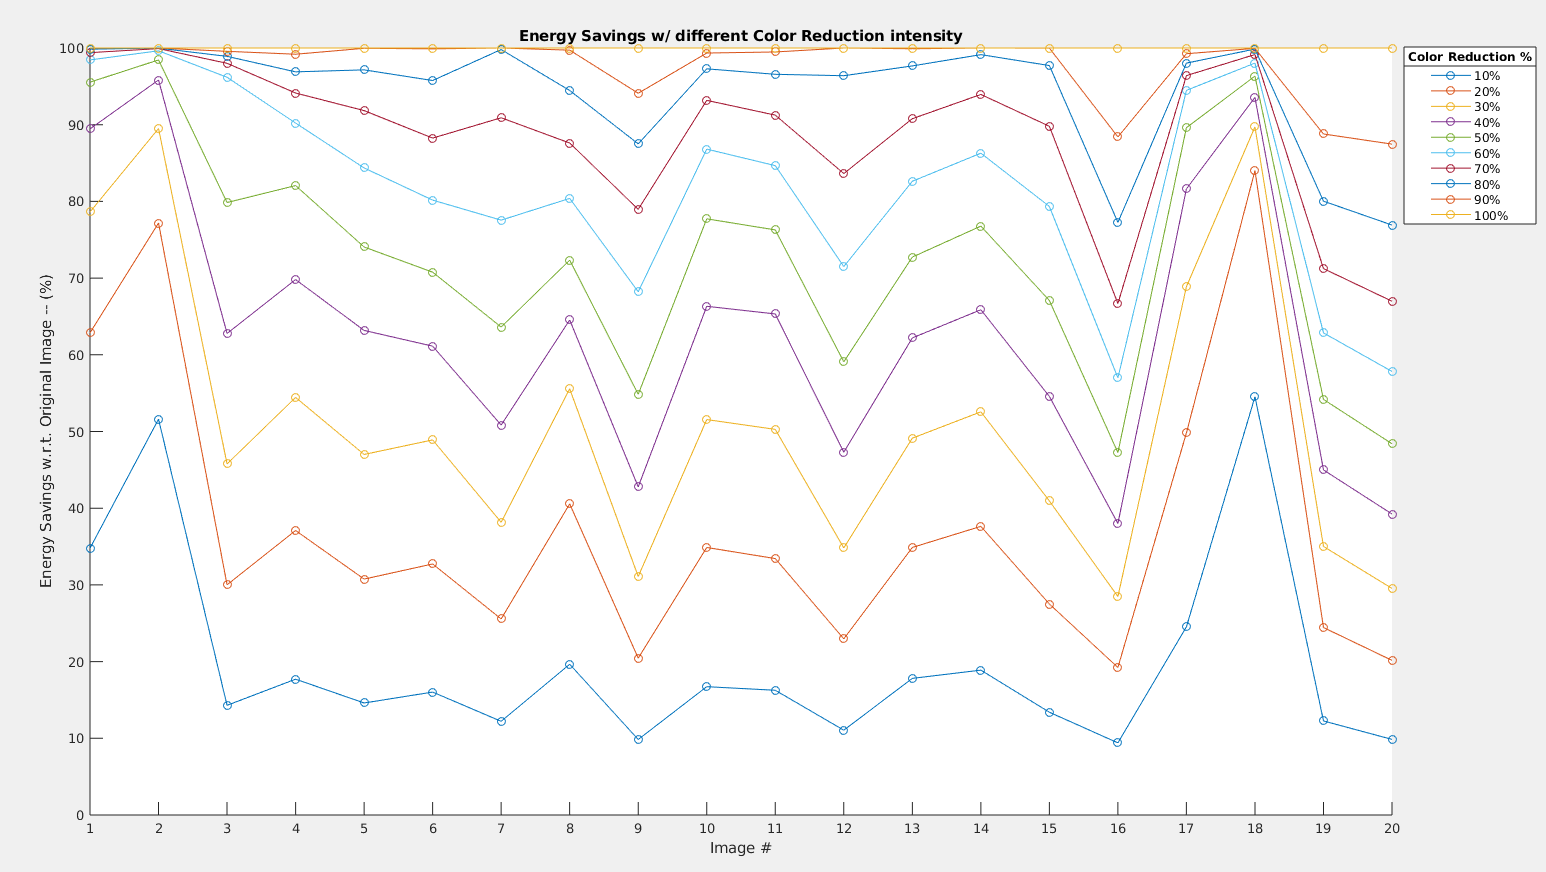
\includegraphics[width=1 \columnwidth]{./screenshots/ColorReductionOverall}
                \caption{
                        \label{fig:ColorReductionOverall}
                        The plot represents, for each of the 15 images (on the $x$ axis) and for each color reduction percentage applied to it (the different curves), the overall power consumption gains obtained.
                }
            \end{figure}

            Starting from image \#16 (i.e. the subset of images representing all the screenshots taken from our PC) we can notice big improvements on the power consumption domain, especially for image \#17 (the MacOS application drawer) and image \#18 (the dark-themed text editor). Especially for this last image, it is clear how a dark background can positively impact the power consumption of emissive displays.

            For this same purpose, we decided to save a comparison image for each degree of color reduction percentage in order to qualitatively assess the quality of the final image. In figure (\ref{fig:color_reduction_20perc_img_11}) we can see what a color reduction of the $20\%$ looks like on an already dark image.

            \begin{figure}[htp]
                \centering
                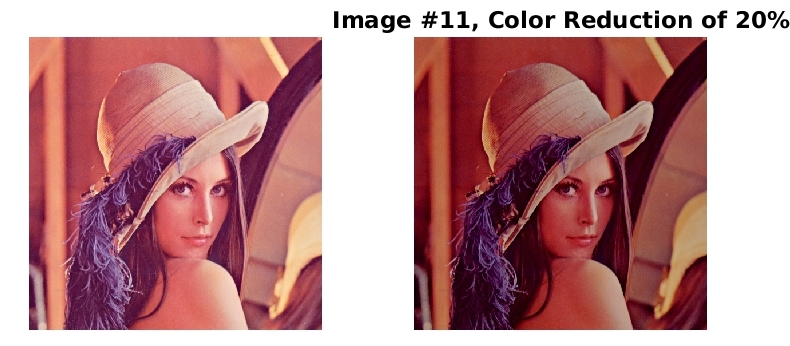
\includegraphics[width=0.6 \columnwidth]{./screenshots/color_reduction_20perc_img_11.jpg}
                \caption{
                        \label{fig:color_reduction_20perc_img_11}
                        On the left the original image, on the right the same image with all colors reduced by the $20\%$. The image is still recognizable and the overall quality is still acceptable. The modified image presents a power consumption gain equal to the $32\%$.
                }
            \end{figure}

            \begin{figure}[htp]
                \centering
                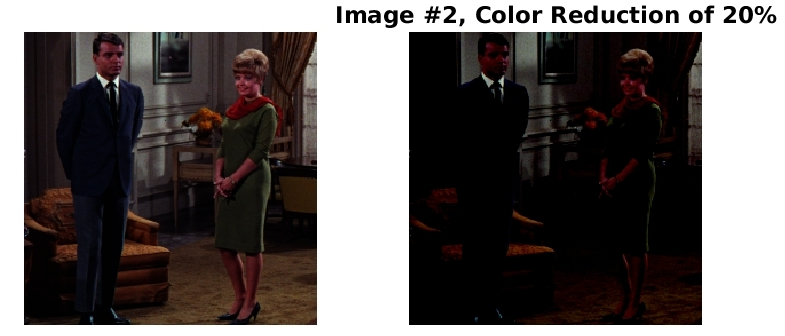
\includegraphics[width=0.6 \columnwidth]{./screenshots/color_reduction_20perc_img_2.jpg}
                \caption{
                        \label{fig:color_reduction_20perc_img_2}
                        On the left the original image, on the right the same image with all colors reduced by the $20\%$. The image is too distorted and the quality loss is unacceptable. This is due to the intrinsic darkness of the original image.
                }
            \end{figure}

            Finally, to evaluate the energy consumption gains alongside a quantitative evaluation of the image distortion, we plotted, for each image in the image set, a graph that shows the trends of both the power consumption and the euclidean (or SSIM) metric. As we can see from figure (\ref{fig:img2_EUCLvSSIM}), each $x$ value corresponds to a different color reduction percentage, on the left $y$ axis we reported the energy savings obtained and on the right $y$ axis we reported the Euclidean Distance (or SSIM) values.

            \begin{figure}[htp]
                \centering
                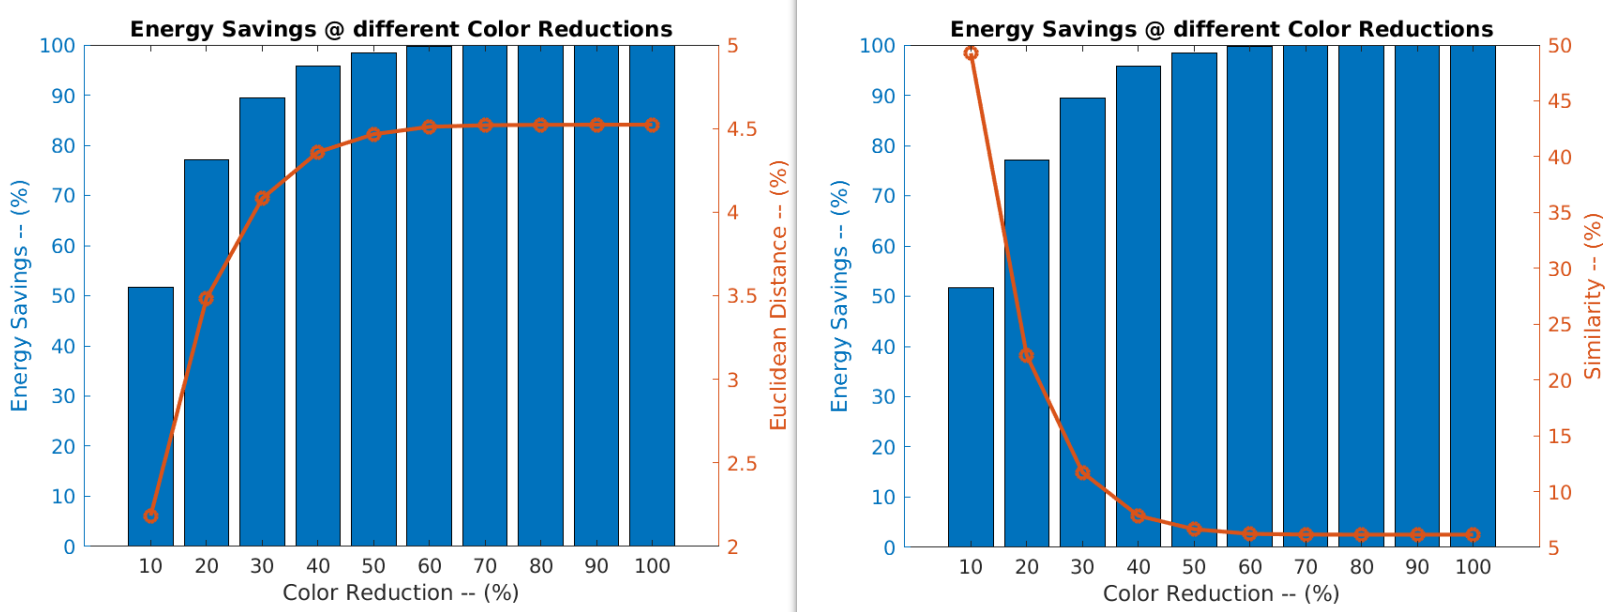
\includegraphics[width=0.8 \columnwidth]{./screenshots/img2_EUCLvSSIM.png}
                \caption{
                        \label{fig:img2_EUCLvSSIM}
                        Two graphs regarding image \#2, representing the tradeoff between the power consumption gains obtained with 10 different color reduction profiles and the two techniques used to assert the image distortion (on the left the Euclidean Distance, on the right the SSIM similarity index).
                }
            \end{figure}

            From this figure we can easily understand that the SSIM technique (used to evaluate the image distortion) is the one that better reflects the real image quality as seen by the human eye. As an example (refer also to figure (\ref{fig:color_reduction_20perc_img_2})): notice that at $20\%$ of color reduction the SSIM index indicates that the similarity of the modified image against the original one is slightly below the $22\%$. By qualitatively comparing the two images we can appreciate in fact the over-distorted condition of the modified image. On the other hand, the Euclidean Distance, for the same color reduction percentage, tops at a $3.45\%$ distance from the original image: this obviously does not reflect the real final distortion perceived on the modified image.

        \subsubsection{Histogram Equalization Plots}
            Similar plots have been made also for the Histogram Equalization image manipulations. For each image of the set, we extracted a figure containing the original image and its related color histogram, compared with the modified image (that has been histogram equalized) and its related color histogram.
            Finally, we made a plot that compares, for each image, the power consumption gains obtained, the Euclidean Distance and the SSIM parameter.

            This summarized plot can be observed in figure (\ref{fig:HistEqOverall}).
            From the left graph (the one representing the power consumption) it is possible to see that some images, for example image \#1, \#2 and the screenshots \#17 and \#18 suffer from an increase of the power consumption up to $130\%$. At the same time, all the other images present a power consumption reduction which is less evident with respect to the Color Reduction technique. However, the similarity of most of the images is between the $40\%$ and the $60\%$, with some images peaking even above the $80\%$. Once again, the Euclidean Distance, especially considering the previous results obtained when evaluating the Color Reduction, cannot be considered as a good metric to evaluate the image distortion as perceived by the human eye.

            \begin{figure}[htp]
                \centering
                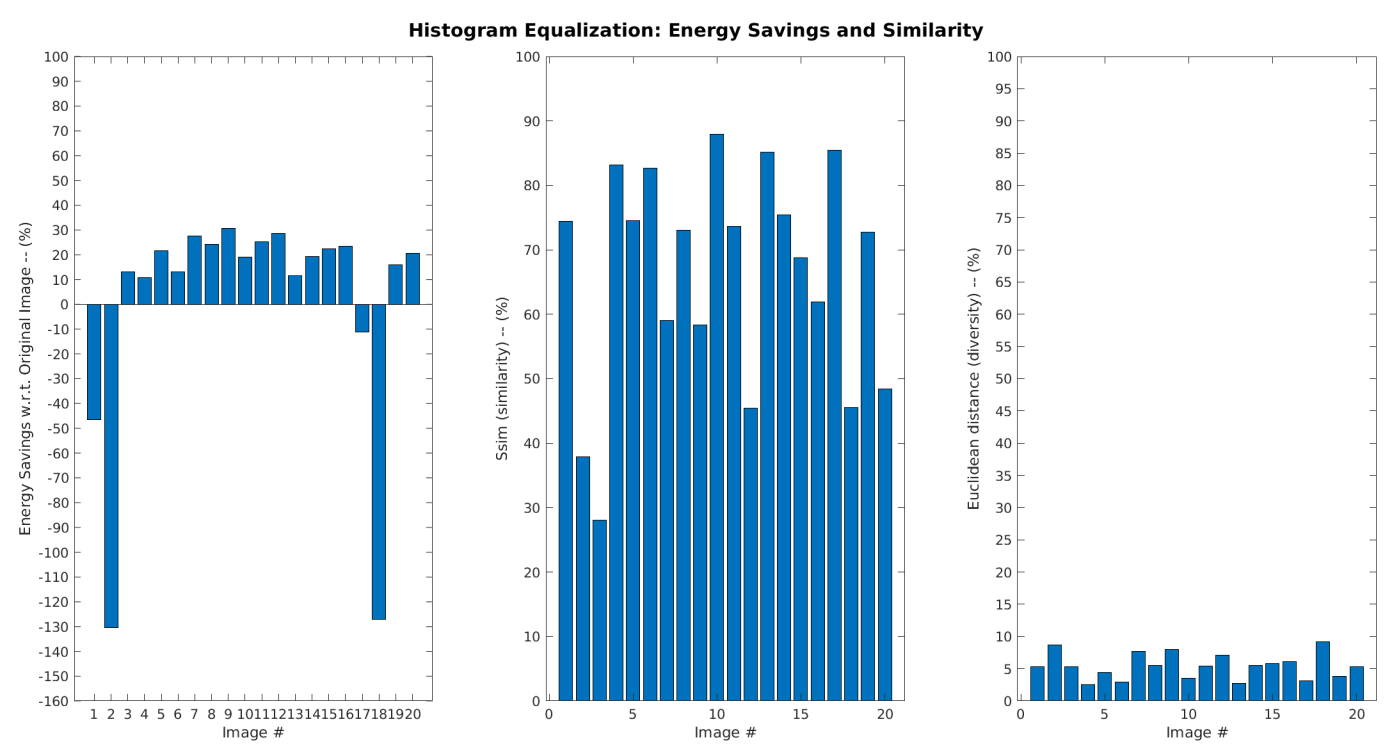
\includegraphics[width=0.8 \columnwidth]{./screenshots/HistEqOverall}
                \caption{
                        \label{fig:HistEqOverall}
                        Summarized plot representing, for each image of the set, the power consumption, the Euclidean Distance and the SSIM parameter obtained after the Histogram Equalization.
                }
            \end{figure}

            From now on, we will discuss some of the most interesting results obtained by considering a single image at a time.
            In figure (\ref{fig:hist_equalization_RGB_img_2}) we can, for example, observe the Histogram Equalization applied to the second image of the entire set: this image demonstrates that the equalization process can in fact increase the power consumption of an image. In this case, we can see that the application of the equalizer "stretches" horizontally the entire histogram: in the original images most of the colors were concentrated on the left half of the histogram, proving the overall darkness of the original image. The equalization "expanded" the concentration of the colors also to the right part of the histogram, occupying also the more bright zones of the histogram (the ones near the value 255).

            \begin{figure}[htp]
                \centering
                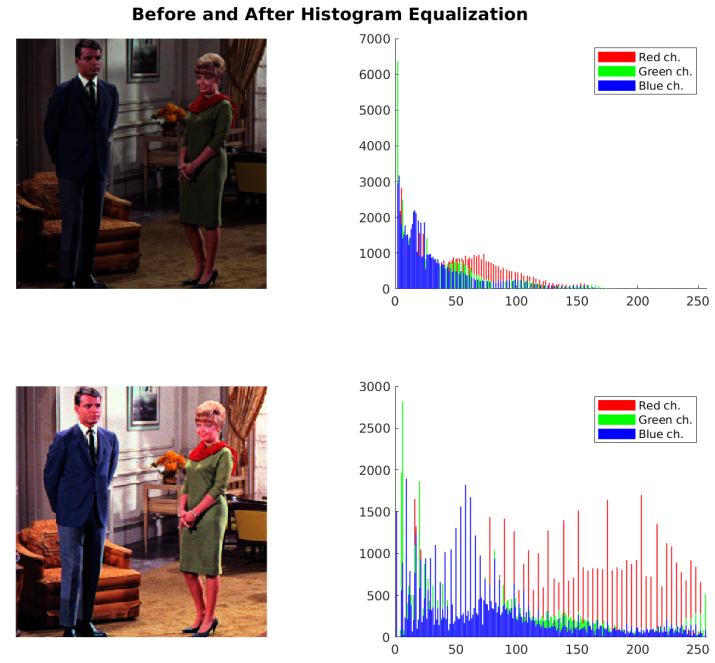
\includegraphics[width=0.6 \columnwidth]{./screenshots/hist_equalization_RGB_img_2}
                \caption{
                        \label{fig:hist_equalization_RGB_img_2}
                        An example of Histogram Equalization that actually increases the power consumption of an image: the color histogram is stretched up to the most bright zones (as a rule of thumb, the more the brightness of the image, the more its power consumption). This image, once equalized, results in a power consumption increased by $130\%$.
                }
            \end{figure}

            An example of a good histogram equalization can be seen in figure (\ref{fig:hist_equalization_RGB_img_13}). Here, the original image (image \#13) presents an histogram which is already "stretched" enough to cover the entire $x$ axis uniformly. The application of the equalization hence stretches even more the histogram, especially for the red channel. As a result, the image appears really similar to the original one, however with darker shadows and an overall better exposure. If we now see the power consumption in the summarizing plot, we can see that image \#13 has a power consumption which is reduced of the $30\%$, which is a very good result considering the overall quality of the final image. Such result suggests that an Histogram Equalization transformation is best suited to images that are overall "equilibrate" in terms of color presence in their related histogram.

            \begin{figure}[htp]
                \centering
                \includegraphics[width=0.6 \columnwidth]{./screenshots/hist_equalization_RGB_img_13}
                \caption{
                        \label{fig:hist_equalization_RGB_img_13}
                        An example of good Histogram Equalization. The image appear nearly the same as the original, but with a power consumption that is reduced by the $30\%$.
                }
            \end{figure}

        \subsubsection{Luminance Reduction Plots}
            In this last section we finally analyze the results obtained when reducing the luminance of an image. The results are overall similar to what we have obtained with the color reduction (the transformations are in fact similar).

            In figure (\ref{fig:LuminanceReductionOverall}) we report a very similar plot (although different in the values represented) to what we already illustrated for the color reduction process.
            In this case, the luminance reduction appears to be "less aggressive" in terms of gains of power consumption.
            For example, for image \#1, we were able to obtain with a $10\%$ of color reduction, a gain in power consumption of the $52\%$. On the other hand, with a $10\%$ of luminance reduction, we obtained a gain in power consumption equal to the $44\%$. Similar reductions are observable also with other images. However, it should be noted that the both plots (\ref{fig:ColorReductionOverall} and \ref{fig:LuminanceReductionOverall}) are really similar in terms of curve trends.

            \begin{figure}[htp]
                \centering
                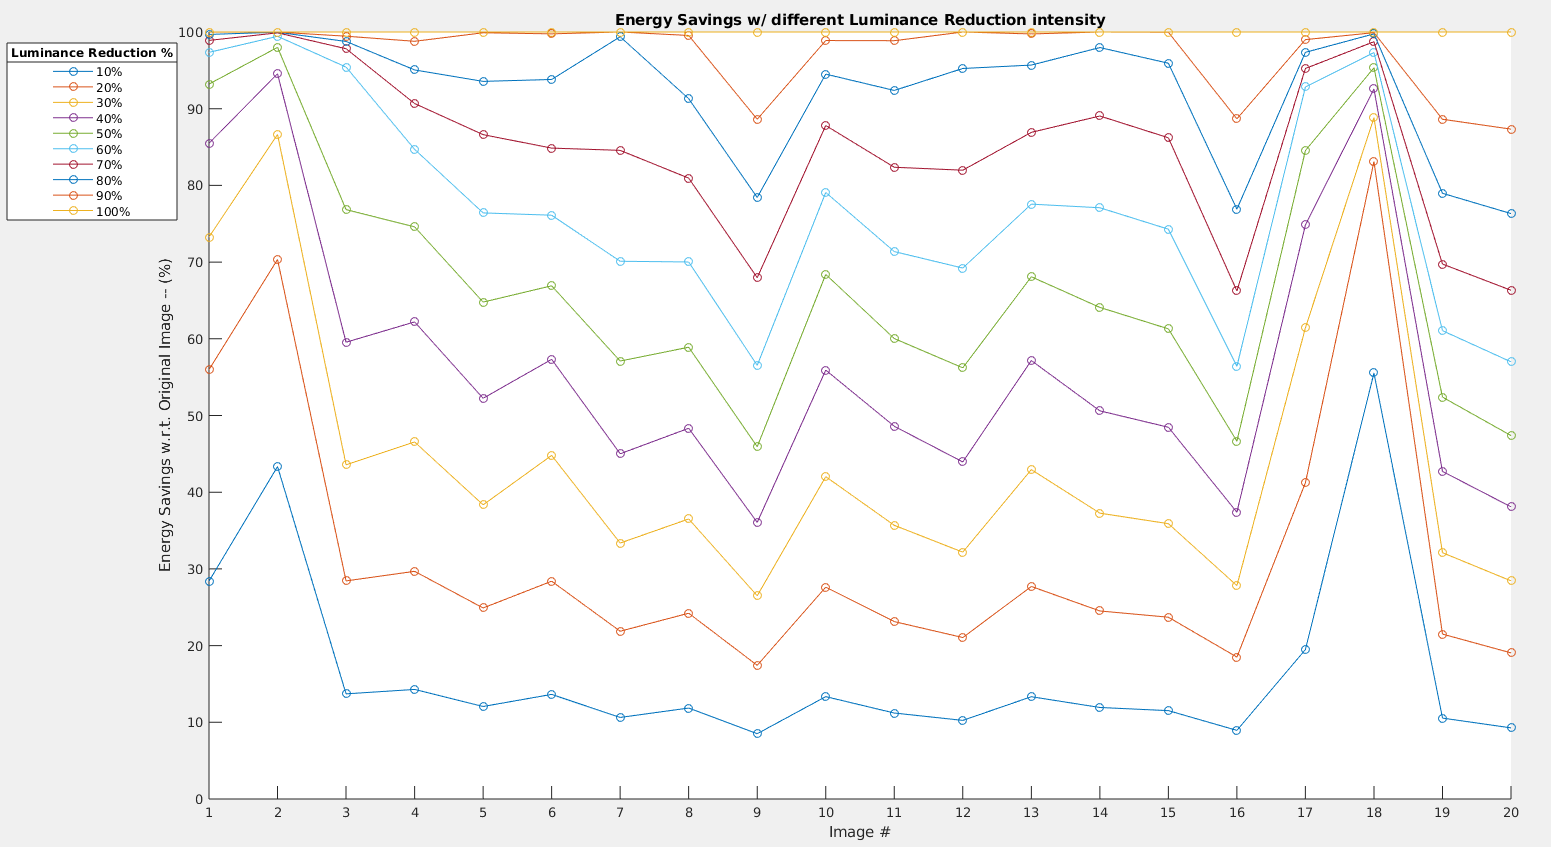
\includegraphics[width=0.8 \columnwidth]{./screenshots/LuminanceReductionOverall}
                \caption{
                        \label{fig:LuminanceReductionOverall}
                        The plot represents, for each of the 15 images (on the $x$ axis) and for each luminance reduction percentage applied to it (the different curves), the overall power consumption gains obtained.
                }
            \end{figure}

            In the following figure (\ref{fig:img11_COLvLUM}) we compared the results obtained with the same image (image \#11) for both color reduction and luminance reduction. From this comparison we can see the differences, small but still significant, between the two techniques. From this comparison the luminance reduction seems to deliver a better image, with colors not too distorted, especially if we compare it against the strong red deviation of the skin color that we find in the color reduced image.

            \begin{figure}[htp]
                \centering
                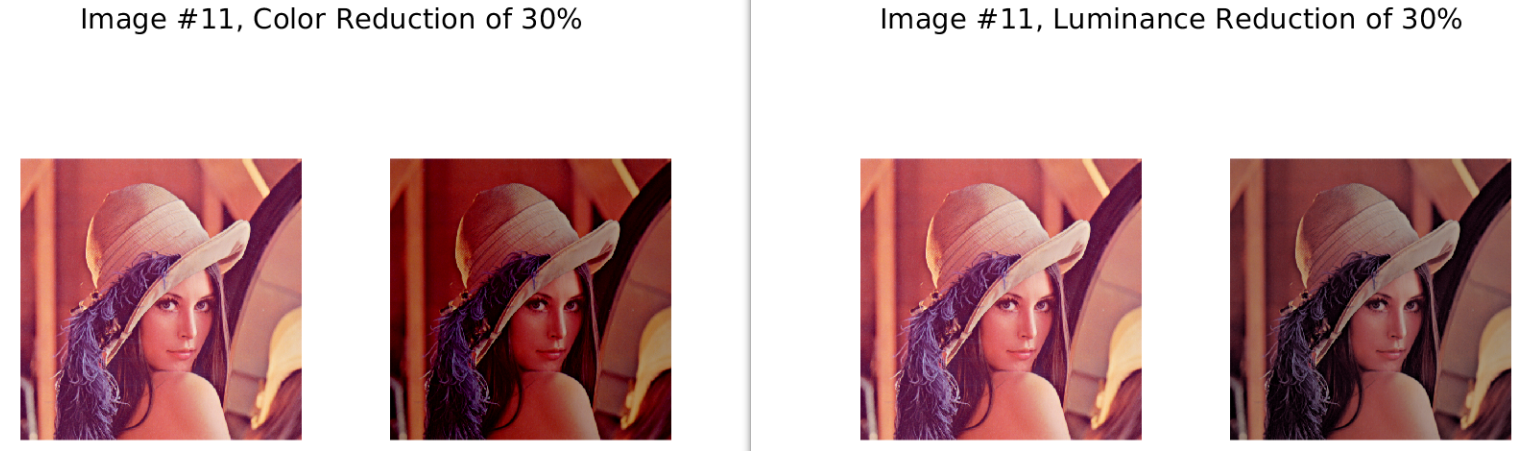
\includegraphics[width=0.6 \columnwidth]{./screenshots/img11_COLvLUM}
                \caption{
                        \label{fig:img11_COLvLUM}
                        Comparison between the Color Reduction and the Luminance Reduction techniques. In this case, the Luminance Reduction delivers colors that are more faithful to the original image.
                }
            \end{figure}

            An interesting behavior has been obtained with the screenshots taken from our PC (image \#18), as we can see from figure (\ref{fig:luminance_reduction_10perc_img_18}) and figure (\ref{fig:ImagePercSavingsBar_LUMRED_SSIM_img_18}).
            From the first picture we can appreciate that a small color reduction does not affect too much the overall look of the dark-theme applied to the application, confirming once again that dark-themes are in fact beneficial when applied to emissive displays.
            Finally, from the second picture we can also appreciate the fact that, once the $20\%$ of reduction threshold is overcome, the trend of the power consumption faces more and more resistivity, suggesting that further luminance reductions will probably impact too much the image quality for very limited gains obtained on the power consumption domain.

            \begin{figure}[htp]
                \centering
                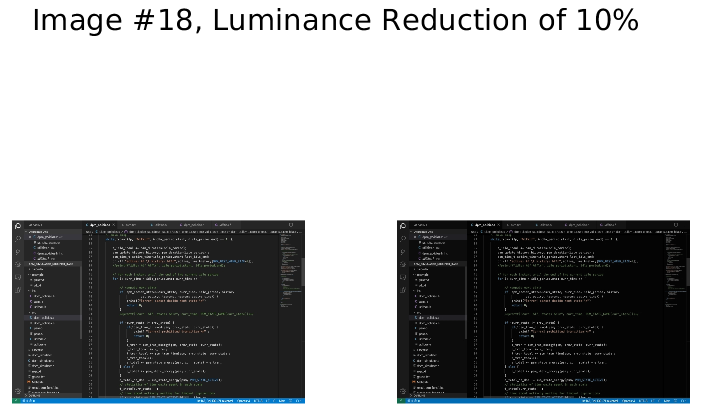
\includegraphics[width=0.6 \columnwidth]{./screenshots/luminance_reduction_10perc_img_18}
                \caption{
                        \label{fig:luminance_reduction_10perc_img_18}
                        A screenshot of an application supporting a dark theme (image \#18).
                }
            \end{figure}

            \begin{figure}[htp]
                \centering
                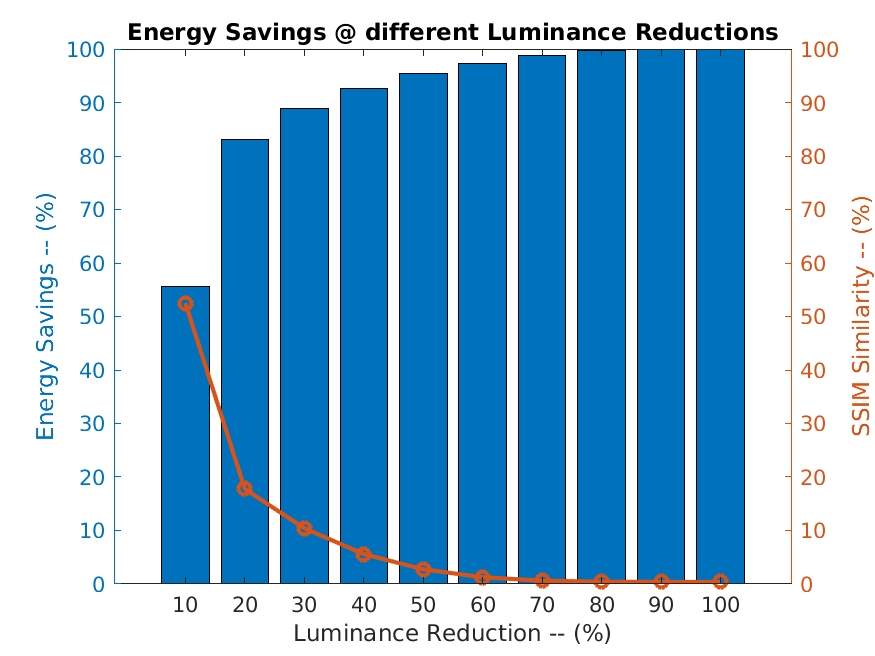
\includegraphics[width=0.6 \columnwidth]{./screenshots/ImagePercSavingsBar_LUMRED_SSIM_img_18}
                \caption{
                        \label{fig:ImagePercSavingsBar_LUMRED_SSIM_img_18}
                        The overall power consumption behavior of the same screenshot of figure (\ref{fig:luminance_reduction_10perc_img_18}). We can see that a luminance reduction of the $10\%$ is sufficient to obtain a power consumption which is reduced up to the $55\%$.
                }
            \end{figure}

        \subsubsection{Conclusions}
        All the results obtained allow us to define some basic approaches to image manipulation. For example, we can infer that the color reduction technique cannot always be applied to all images: some images (like the one depicted in figure (\ref{fig:color_reduction_20perc_img_2})) suffer from distortion even if affected by small manipulations.
        
        In general, all of the three techniques we tested cannot be applied by default on all images without exploring the tradeoffs and evaluating carefully the results obtained image-per-image. Some of them provide in fact very good results on some images while very poor on other ones.
        Hence, it is not possible to define a "golden" manipulation technique able to return good results on the power consumption domain and poor image distortion for all the images.
        
        If we consider the Color Reduction technique, a good policy will evaluate carefully the original image power consumption (tightly related to the overall darkness of an image), defining a threshold that, if surpassed, will resort to the application of the technique. Hence, images like image \#1 and \#2 will be kept in their original form, meanwhile images like image \#9 will be color reduced.

        A similar approach can be taken also considering the histogram equalization: from our experiments it is clear that static images like the screenshots obtained from our PC will suffer from a heavily degraded image quality if the equalization is applied. Histogram Equalization is better suited for photos and videos, where the overall image does not have an intrinsic "flat" or "unbalanced" histogram. Hence, we can apply some sort of filtering of the input image to avoid to apply this transformations to images we know in advance will be too distorted or will lead to an increased power consumption.

        Finally, the luminance reduction technique demonstrated to be very effective if applied on our screenshots, where the majority of the image area is predominantly light or dark.
        Once again, we can think of a good automatic policy applying an histogram equalization on multimedia applications (like video-streaming ones) and luminance reduction on static applications (like text editors, spreadsheets and textual webpages).

%   _____           _     ___
%  |  __ \         | |   |__ \
%  | |__) |_ _ _ __| |_     ) |
%  |  ___/ _` | '__| __|   / /
%  | |  | (_| | |  | |_   / /_
%  |_|   \__,_|_|   \__| |____|
%
\section{Part 2: Interfacing w/ an external OLED display | Image manipulation on-the-edge}
    For this second part of the laboratory we were required to use some additional equipment to load and test our set of images on a real emissive display. We were provided, in fact, with an \emph{Arduino UNO} board and an OLED Display by \emph{Newhaven Display} connected to it.
    The goal is to asses the real impact on visual quality for the modifications made in the first part of the laboratory. Finally, this process allowed us also to learn how to interface our \texttt{MATLAB} environment with an 8-bit microcontroller, especially from the point of view of the serial interconnection protocol.
    In the following sections we will discuss both sides of the project: the \texttt{MATLAB} related one and the \emph{Arduino} related one. As a final task, we will discuss the peculiarities observed when displaying the images on the OLED display and our attempt to manipulate the images by directly leverage the microcontroller logic.

    \subsection{The \texttt{MATLAB} Script}
        In the following sections we will discuss the \texttt{MATLAB} script (\texttt{BoardUpload.m}) used to send the images to the \emph{Arduino} microcontroller.

        \subsubsection{Image Manipulation Prior Transfer}
            Before sending the images directly to the \emph{Arduino} board, some modifications to each image have to be made considering the characteristics of the provided OLED display.
            This display has in fact a resolution of 128x128 pixels and its controller handles the data of each pixel not in a "classical" \texttt{RGB} schema, but on an "inverted" \texttt{BGR} schema. Finally, each pixel, which on classical displays is encoded into the 3 \texttt{RGB} 8-bit channels, is here encoded into 6-bit channels.

            Our script starts by loading into memory the image that has to be sent to the microcontroller. The image is then resized to match the 128x128 resolution of the OLED display. After that, each of the 3 available channels is then transformed from an 8-bit notation into a 6-bit notation (to do that, a simple shift right operation by two positions has to be performed).

            Now the image (if no additional transformation has to be done on the PC side) is ready to be sent to the microcontroller. In the following section we explain how this procedure is handled from the \texttt{MATLAB} perspective.

        \subsubsection{Serial Communication}
            The \emph{Arduino UNO} board communicates using the same USB cable it uses as a power supply: the communication is serial and the \texttt{UART} protocol has to be used.
            \texttt{MATLAB} already provides the \texttt{serial()} method to correctly configure and interface our PC with additional Serial hardware like the one we have.
            To create a serial connection it is firstly mandatory to acquire the serial port \emph{Arduino} is connected to: in our case, using a \emph{Windows} PC, the serial port was called \texttt{COM3}.

            While defining the serial connection using the \texttt{serial()} method we need to also define the classical configuration parameters a \texttt{UART} connection requires like the \emph{BaudRate}, the presence of the parity bit (none, odd, even, mark, space), the number of data bits (5, 6, 7 or 8-bit), the byte order (big/little endian) etc... In our case, the default configuration provided by the method was sufficient: the only modification to be done was the one related to the BaudRate, configured at 115200 \texttt{BAUD}.

            After that, it is only matter to open the connection using the \texttt{fopen()} method: if the serial port is not busy or occupied by another process, the connection will allow us to send the bytes representing our image to the \emph{Arduino} board.
            Just after opening the connection we invoke the function \texttt{send\_image(file\_pointer, img\_R, img\_G, img\_B)} that we defined in order to automatically handle all the byte-transferring process.
            When invoking it, we complete the last manipulation to the image needed to interface properly with the display controller: we swap the \texttt{RGB} channels into the new \texttt{BGR} notation.
            This function is defined in the \texttt{send\_image.m} script: by leveraging the \texttt{fwrite()} function we send, pixel after pixel, the 3 bytes corresponding to the 3 channels that compose each pixel (i.e. at each iteration only one pixel is sent, hence requiring 128x128 iterations to send a complete image).

    \subsection{The Arduino Program}
        As a second task necessary to complete the image transfer it is required to implement the code that allows the \emph{Arduino} board to correctly handle the reception of the image from the serial connection initialized by the \texttt{MATLAB} script.
        The provided code contains a set of high-level library functions that allow to complete some basic operations and to correctly interface the board with the display controller.

        The \emph{Arduino} sketch starts by the definition of some pre-processor commands that allow us to compile (or not) some sections of the code (we will discuss them later).
        Also, some variables are defined, like the \texttt{rcv\_data[8]} array of \texttt{char}s that is used to load into memory the 8 different Bytes received from the serial connection.
        The first operation completed after the reset of the board is the setup of the interconnection to the OLED display and the setup of the display controller. Once these operations completed, we can set the starting position (i.e. the display cursor) from which the images will be shown on the physical display.

        Finally, after this setup section, the code loops indefinitely until a serial connection is started by the \texttt{MATLAB} script (that will trigger the \texttt{serialEvent()} interrupt routine).

        \subsubsection{Image Reception}
            Now, assuming a byte has been sent by the \texttt{MATLAB} script through the serial connection, the microcontroller will start to execute the \texttt{serialEvent()} routine.
            Before explaining what the code implemented will do next it is necessary to explain how an \emph{Arduino} board "reads" the data sent through the serial port. In fact, each character sent through the serial connection is interpreted like an \texttt{UTF-8} 8-bit character. If we now recall that the \texttt{MATLAB} script sends 8 characters at a time (corresponding to a single Byte of a single channel) we can understand that each one of these characters will be interpreted by \emph{Arduino} like and 8-bit character itself. Hence, if we send the "\texttt{0100|1001}" Byte using \texttt{MATLAB}, \emph{Arduino} will interpret this Byte as an array of 8 different Bytes, where each element of the array represents the ASCII code either of the character '\texttt{0}' or of the character '\texttt{1}'.

            Hence, our \emph{Arduino} code will read the entire sequence of 8 characters sent over the serial connection and place it into the \texttt{rcv\_data[8]} array of \texttt{char}s. That done, we start a loop of 8 iterations in order to "translate" each ASCII code received into the actual bit value and push this value into a single \texttt{char} variable (called \texttt{data}) containing the reconstructed 8-bit sequence.

            Once the sequence reconstructed, it is sent to the display controller using the \texttt{OLED\_Data\_128128RGB(data)} function. By doing that, we have transferred the first Byte, corresponding to one of the three Bytes needed to complete a single pixel.

            In the following figure (\ref{fig:OriginalImageArduino}) we can see the same image which is color reduced by \texttt{MATLAB} on the left side of the screen and in its original form on the right side of the screen.

            \begin{figure}[htp]
                \centering
                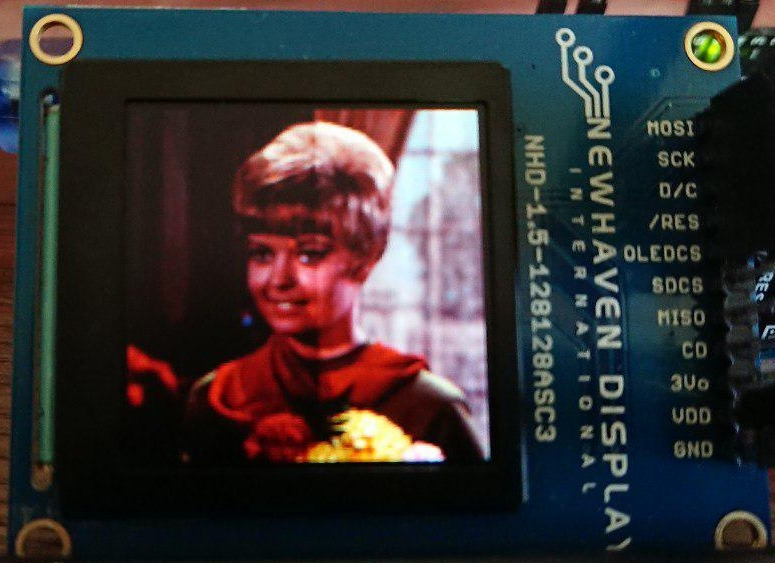
\includegraphics[width=0.4 \columnwidth]{./screenshots/OriginalImageArduino}
                \caption{
                        \label{fig:OriginalImageArduino}
                        The OLED display representing the same image color reduced by \texttt{MATLAB} on the left side of the screen and in its original form on the right side of the screen. The image was loaded in around 20-30 seconds.
                }
            \end{figure}

        \subsubsection{Image Manipulation}

            Since the Bytes sent to \emph{Arduino} on the serial port cannot be stored in RAM because of its limited capacity, it is necessary to modify the single Bytes \emph{on-the-fly} just after reception and before sending them again to the display controller.

            To do that we added a piece of code, protected by the pre-processor directive \texttt{IMG\_EDIT} in order to mask or unmask the code prior compilation.
            We decided to opt for a color manipulation technique, similar to the first manipulation technique we mentioned for the first part of the report. Also in this case, we defined a constant called \texttt{COLOR\_REDUCTION\_PERC} representing the percentage of reduction we want to apply to each channel of the image.

            Since the color reduction must be applied \emph{on-the-fly}, the computation is done in the \texttt{serialEvent()} routine: here the reduction value is subtracted to the original value and the new color reduced \texttt{data} variable is sent to the display controller. In the following picture (\ref{fig:ColorReductionComparison}) we reported a photo of the OLED display showing a comparison between our image, which is color reduced by \texttt{MATLAB} (on the right side of the screen) and the same image but color reduced \emph{on-the-fly} by \emph{Arduino} (on the left side of the screen).
            From this picture it is possible to notice the clear distortion caused by the color reduction applied at run-time to the original image, making such technique not feasible for everyday operations.

            \begin{figure}[htp]
                \centering
                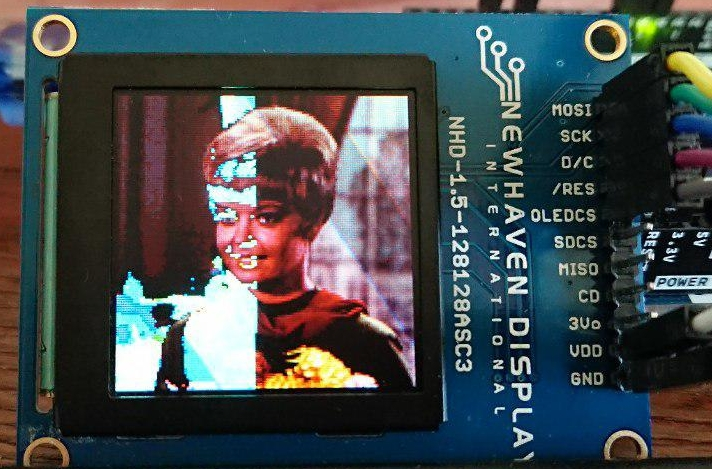
\includegraphics[width=0.4 \columnwidth]{./screenshots/ColorReductionComparison}
                \caption{
                        \label{fig:ColorReductionComparison}
                        The OLED display representing the same image with the two different color reductions applied: on the left the color reduction ($10\%$) done by \emph{Arduino}, on the right the color reduction ($10\%$) done by \text{MATLAB}.
                }
            \end{figure}

\end{document}